\documentclass[12pt,a4paper]{article}
\usepackage[a4paper, margin=0.8in, headheight=14pt]{geometry}
\usepackage{fontspec}
\usepackage{unicode-math}
\setmainfont{TeX Gyre Pagella}
\setmonofont[Scale=0.88]{TeX Gyre Cursor}
\setmathfont{Latin Modern Math}

\usepackage{xcolor}
\usepackage{colortbl}
\usepackage{titlesec}
\usepackage{enumitem}
\usepackage{tabularx}
\usepackage{booktabs}
\usepackage{array}
\usepackage{amsmath}
\allowdisplaybreaks
\usepackage{tikz}
\usetikzlibrary{shapes.geometric, arrows.meta, positioning, calc, fit, decorations.pathreplacing, patterns}
\usepackage{tcolorbox}
\tcbuselibrary{skins, breakable}
\usepackage{hyperref}
\usepackage{fancyhdr}
\usepackage{graphicx}
\usepackage{microtype}
\hyphenpenalty=10000
\exhyphenpenalty=10000
\sloppy
\usepackage{caption}
\usepackage{setspace}
\usepackage{multirow}
\usepackage{tocloft}

% ─── Q&A helper ────────────────────────────────────────────────────────────────
\newcommand{\Q}[1]{\textbf{#1}\par\noindent\ignorespaces}

% ─── Colour Palette ────────────────────────────────────────────────────────────
\definecolor{myred}{RGB}{196,30,58}
\definecolor{mydark}{RGB}{30,30,50}
\definecolor{mygreen}{RGB}{14,120,80}
\definecolor{myteal}{RGB}{0,130,140}
\definecolor{myamber}{RGB}{220,130,20}
\definecolor{mypurple}{RGB}{90,40,140}
\definecolor{mygray}{RGB}{248,249,251}
\definecolor{mgframe}{RGB}{215,220,230}
\definecolor{watermark}{RGB}{145,150,170}
\definecolor{hdrred}{RGB}{250,232,235}
\definecolor{hdrgreen}{RGB}{220,244,233}
\definecolor{hdrteal}{RGB}{220,242,244}
\definecolor{hdramber}{RGB}{253,242,215}
\definecolor{hdrpurple}{RGB}{238,228,255}
\definecolor{hdrgray}{RGB}{238,240,245}
\definecolor{rowalt}{RGB}{250,251,253}

% ─── Section Formatting ────────────────────────────────────────────────────────
\titleformat{\section}
  {\large\bfseries\color{myred}}{\thesection.}{0.5em}{}
  [\vspace{1pt}{\color{myred}\rule{\linewidth}{0.8pt}}]
\titleformat{\subsection}
  {\normalsize\bfseries\color{myteal}}{\thesubsection}{0.5em}{}
\titlespacing*{\section}{0pt}{18pt}{7pt}
\titlespacing*{\subsection}{0pt}{11pt}{4pt}

% ─── Paragraph ─────────────────────────────────────────────────────────────────
\setlength{\parindent}{0pt}
\setlength{\parskip}{4pt}

% ─── TOC Styling ───────────────────────────────────────────────────────────────
\renewcommand{\cfttoctitlefont}{\large\bfseries\color{myred}}
\renewcommand{\cftaftertoctitle}{\par\noindent{\color{myred}\rule{\linewidth}{0.8pt}}}
\setlength{\cftbeforetoctitleskip}{0pt}
\setlength{\cftaftertoctitleskip}{6pt}
\renewcommand{\cftsecfont}{\normalsize\bfseries\color{mydark}}
\renewcommand{\cftsecpagefont}{\normalsize\bfseries\color{mydark}}
\renewcommand{\cftsecleader}{\cftdotfill{\cftdotsep}}
\setlength{\cftbeforesecskip}{7pt}
\renewcommand{\cftsubsecfont}{\small\color{mydark}}
\renewcommand{\cftsubsecpagefont}{\small\color{mydark}}
\setlength{\cftbeforesubsecskip}{3pt}
\setlength{\cftsubsecindent}{1.4em}

% ─── Table helpers ─────────────────────────────────────────────────────────────
\renewcommand{\arraystretch}{1.45}
\setlength{\tabcolsep}{6pt}
\arrayrulecolor{mydark}
\newcolumntype{B}[1]{>{\small\bfseries\raggedright\arraybackslash}m{#1}}
\newcolumntype{Y}{>{\small\raggedright\arraybackslash}X}
\renewcommand{\tabularxcolumn}[1]{m{#1}}

% ─── Header / Footer ───────────────────────────────────────────────────────────
\pagestyle{fancy}
\fancyhf{}
\fancyhead[L]{\small\color{myred}\textbf{EC303}\;\color{mydark}--- Signals and System}
\fancyhead[R]{\small\color{myteal}\textbf{Module 4 Notes}}
\fancyfoot[C]{\small\color{mydark}\thepage}
\fancyfoot[R]{\small\color{watermark}\textit{\copyright\ Biraj}}
\renewcommand{\headrulewidth}{0.5pt}
\renewcommand{\footrulewidth}{0.3pt}

% ─── Hyperref ──────────────────────────────────────────────────────────────────
\hypersetup{
  colorlinks=true, linkcolor=myteal, urlcolor=myteal,
  pdfauthor={Biraj Sarkar (CGEC)},
  pdftitle={EC303 --- Module 4 Notes: Laplace and Z-Transforms}
}

% ─── tcolorbox styles ──────────────────────────────────────────────────────────
\tcbset{
  tikzbox/.style={
    colback=mygray, colframe=mgframe, boxrule=0.6pt, arc=4pt,
    left=8pt, right=8pt, top=6pt, bottom=6pt,
    colbacktitle=mgframe, coltitle=mydark,
    fonttitle=\small\bfseries
  },
  defbox/.style={
    colback=hdrgreen, colframe=mygreen, boxrule=0.8pt, arc=4pt,
    left=9pt, right=9pt, top=6pt, bottom=6pt,
    colbacktitle=mygreen, coltitle=white,
    fonttitle=\small\bfseries
  },
  formulabox/.style={
    colback=hdrteal, colframe=myteal, boxrule=0.8pt, arc=4pt,
    left=9pt, right=9pt, top=6pt, bottom=6pt,
    colbacktitle=myteal, coltitle=white,
    fonttitle=\small\bfseries
  },
  examplebox/.style={
    colback=hdramber, colframe=myamber, boxrule=0.8pt, arc=4pt,
    left=9pt, right=9pt, top=6pt, bottom=6pt,
    colbacktitle=myamber, coltitle=white,
    fonttitle=\small\bfseries
  },
  masonbox/.style={
    colback=hdrpurple, colframe=mypurple, boxrule=0.8pt, arc=4pt,
    left=9pt, right=9pt, top=6pt, bottom=6pt,
    colbacktitle=mypurple, coltitle=white,
    fonttitle=\small\bfseries
  },
  exambox/.style={
    colback=hdrpurple, colframe=mypurple, boxrule=1pt, arc=5pt,
    left=10pt, right=10pt, top=8pt, bottom=8pt,
    colbacktitle=mypurple, coltitle=white,
    fonttitle=\bfseries,
    breakable, title after break={\textbf{Frequently Asked / Viva Questions (contd.)}}
  }
}

\tcbset{breakable}
\tcbset{after={\color{black}}}

% ─── TikZ Global Styles ────────────────────────────────────────────────────────
\tikzset{
  sysblock/.style={draw=myteal, fill=hdrteal, thick, rectangle, rounded corners=3pt, minimum height=1cm, minimum width=2.4cm, align=center, font=\small\bfseries},
  circnode/.style={draw=myred, fill=hdrred, circle, thick, inner sep=1.5pt, font=\small\bfseries},
  arrowline/.style={-{Latex[length=2.5mm]}, thick, color=mydark},
  dashline/.style={thick, dashed, color=myteal}
}

% ─── Document ──────────────────────────────────────────────────────────────────
\begin{document}

% ─── Title Block ───────────────────────────────────────────────────────────────
\begin{center}
  {\Large\bfseries\color{myred} EC303 --- Signals and System}\\[4pt]
  {\large\bfseries\color{mydark} Module 4: Evolution of Transforms, Laplace \& Z-Transforms}\\[3pt]
  {\small\color{watermark} Prepared by \textbf{Biraj Sarkar (CGEC)} $\cdot$ MAKAUT B.Tech ECE (2023--27)}\\[2pt]
  {\small\color{watermark} Authoritative Syllabus-Aligned Notes}
\end{center}
\vspace{-4pt}
\noindent{\color{myred}\rule{\linewidth}{1.2pt}}

% ─── Table of Contents ─────────────────────────────────────────────────────────
\tableofcontents
\vspace{10pt}
\noindent{\color{mgframe}\rule{\linewidth}{0.6pt}}

% ───────────────────────────────────────────────────────────────────────────────
\section{Evolution of Integral Transforms}
% ───────────────────────────────────────────────────────────────────────────────

\subsection{Limitations of the Fourier Transform}
The Continuous-Time Fourier Transform (CTFT) requires Dirichlet conditions to converge, fundamentally demanding that the signal be absolutely integrable:
\begin{equation}
  \int_{-\infty}^{\infty} |x(t)| dt < \infty
\end{equation}
Consequently, many vital engineering signals cannot be transformed directly using standard CTFT without resorting to distributions or impulse trains:
\begin{enumerate}[topsep=2pt, itemsep=2pt]
  \item Growing exponentials: $x(t) = e^{at} u(t)$ with $a > 0$ (unstable system responses).
  \item Signals of infinite energy and non-decaying nature (e.g., polynomial ramps $t^n u(t)$).
  \item Systems with non-zero initial conditions (differential equations with initial stored energy).
\end{enumerate}

\subsection{Generalization to the Laplace Transform (Continuous Domain)}
To ensure convergence for signals that grow or do not decay, we introduce an exponential damping factor $e^{-\sigma t}$ ($\sigma \in \mathbb{R}$) prior to computing the Fourier transform:
\begin{align}
  \mathcal{L}\{x(t)\} &= \mathcal{F}\{x(t) e^{-\sigma t}\} = \int_{-\infty}^{\infty} \big[x(t) e^{-\sigma t}\big] e^{-j\omega t} dt \\
  &= \int_{-\infty}^{\infty} x(t) e^{-(\sigma + j\omega) t} dt
\end{align}
Defining the \textbf{complex frequency} variable $s \triangleq \sigma + j\omega \in \mathbb{C}$, we arrive directly at the \textbf{Bilateral Laplace Transform}:
\begin{equation}
  X(s) = \int_{-\infty}^{\infty} x(t) e^{-st} dt
\end{equation}
The Fourier transform is simply the Laplace transform evaluated along the imaginary axis ($s = j\omega$, i.e., $\sigma = 0$):
\begin{equation}
  X(j\omega) = \left. X(s) \right|_{s = j\omega} \quad (\text{provided the } j\omega\text{-axis lies within the ROC})
\end{equation}

\subsection{Generalization to the Z-Transform (Discrete Domain)}
Similarly, the Discrete-Time Fourier Transform (DTFT) requires absolute summability $\sum |x[n]| < \infty$. By applying a radial damping factor $r^{-n}$ ($r > 0$) to $x[n]$:
\begin{align}
  \mathcal{Z}\{x[n]\} &= \text{DTFT}\{x[n] r^{-n}\} = \sum_{n=-\infty}^{\infty} \big(x[n] r^{-n}\big) e^{-j\Omega n} \\
  &= \sum_{n=-\infty}^{\infty} x[n] \big(r e^{j\Omega}\big)^{-n}
\end{align}
Defining the complex variable $z \triangleq r e^{j\Omega} \in \mathbb{C}$, we obtain the \textbf{Bilateral Z-Transform}:
\begin{equation}
  X(z) = \sum_{n=-\infty}^{\infty} x[n] z^{-n}
\end{equation}
The DTFT is simply the Z-transform evaluated on the \textbf{unit circle} ($|z| = r = 1$, i.e., $z = e^{j\Omega}$):
\begin{equation}
  X(e^{j\Omega}) = \left. X(z) \right|_{z = e^{j\Omega}} \quad (\text{provided the unit circle lies within the ROC})
\end{equation}

\begin{tcolorbox}[tikzbox, title={\textbf{TikZ Schematic: Mapping Between \texorpdfstring{$s$}{s}-Plane and \texorpdfstring{$z$}{z}-Plane (\texorpdfstring{$z = e^{s T_s}$}{z = e^sTs})}}]
\begin{center}
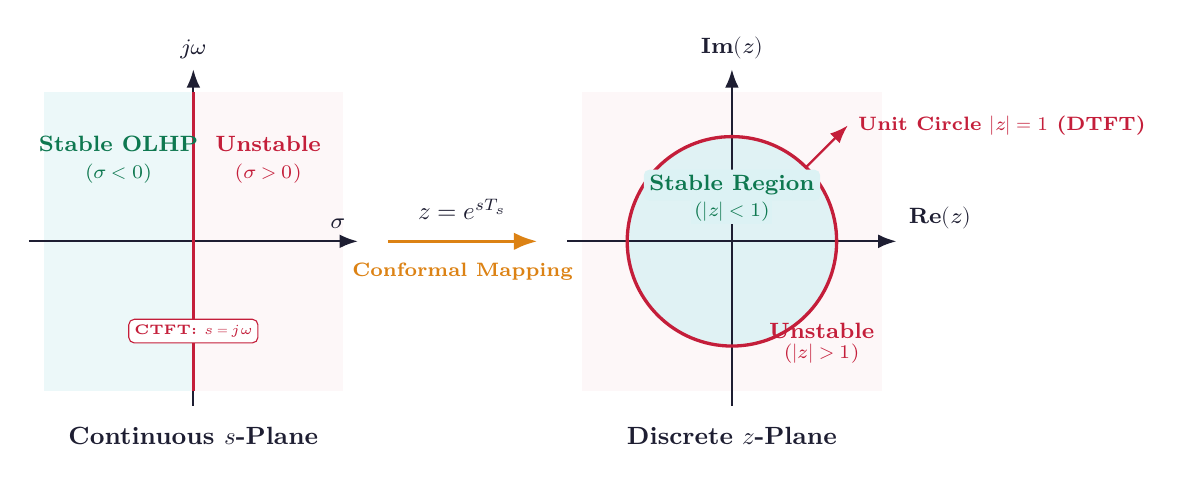
\begin{tikzpicture}[>=Latex, scale=0.95, font=\small]
  % ─── s-Plane (Continuous-Time) ───
  \begin{scope}[xshift=0cm]
    \fill[hdrteal, opacity=0.55] (-2.0,-2.0) rectangle (0,2.0);
    \fill[hdrred, opacity=0.35] (0,-2.0) rectangle (2.0,2.0);
    \draw[->, thick, color=mydark] (-2.2,0) -- (2.2,0) node[above left=1pt, font=\footnotesize\bfseries] {$\sigma$};
    \draw[->, thick, color=mydark] (0,-2.2) -- (0,2.3) node[above, font=\footnotesize\bfseries] {$j\omega$};
    \draw[very thick, myred] (0,-2.0) -- (0,2.0);
    \node[color=mygreen, font=\footnotesize\bfseries] at (-1.0,1.3) {Stable OLHP};
    \node[color=mygreen, font=\scriptsize] at (-1.0,0.9) {($\sigma < 0$)};
    \node[color=myred, font=\footnotesize\bfseries] at (1.0,1.3) {Unstable};
    \node[color=myred, font=\scriptsize] at (1.0,0.9) {($\sigma > 0$)};
    \node[draw=myred, fill=white, rounded corners=2pt, inner sep=2pt, font=\tiny\bfseries, text=myred] at (0,-1.2) {CTFT: $s = j\omega$};
    \node[below=4pt, font=\small\bfseries, color=mydark] at (0,-2.2) {Continuous $s$-Plane};
  \end{scope}

  % ─── Conformal Mapping Transition Arrow ───
  \draw[->, very thick, myamber, -{Latex[length=3mm]}] (2.6, 0) -- (4.6, 0)
    node[midway, above=4pt, font=\small\bfseries, color=mydark] {$z = e^{s T_s}$}
    node[midway, below=4pt, font=\scriptsize\bfseries, color=myamber] {Conformal Mapping};

  % ─── z-Plane (Discrete-Time) ───
  \begin{scope}[xshift=7.2cm]
    \fill[hdrred, opacity=0.35] (-2.0,-2.0) rectangle (2.0,2.0);
    \fill[hdrteal, opacity=0.85] (0,0) circle (1.4cm);
    \draw[->, thick, color=mydark] (-2.2,0) -- (2.2,0) node[above right=1pt, font=\footnotesize\bfseries] {$\text{Re}(z)$};
    \draw[->, thick, color=mydark] (0,-2.2) -- (0,2.3) node[above, font=\footnotesize\bfseries] {$\text{Im}(z)$};
    \draw[very thick, myred] (0,0) circle (1.4cm);
    \node[fill=hdrteal, rounded corners=2pt, inner sep=2pt, text=mygreen, font=\footnotesize\bfseries] at (0, 0.75) {Stable Region};
    \node[fill=hdrteal, inner sep=1pt, text=mygreen, font=\scriptsize] at (0, 0.40) {($|z| < 1$)};
    \node[color=myred, font=\footnotesize\bfseries] at (1.2, -1.2) {Unstable};
    \node[color=myred, font=\scriptsize] at (1.2, -1.5) {($|z| > 1$)};
    \draw[->, myred, thick] (0.99, 0.99) -- (1.55, 1.55) node[right, font=\scriptsize\bfseries, color=myred] {Unit Circle $|z|=1$ (DTFT)};
    \node[below=4pt, font=\small\bfseries, color=mydark] at (0,-2.2) {Discrete $z$-Plane};
  \end{scope}
\end{tikzpicture}
\end{center}
\end{tcolorbox}

% ───────────────────────────────────────────────────────────────────────────────
\section{The Laplace Transform}
% ───────────────────────────────────────────────────────────────────────────────

\subsection{Bilateral and Unilateral Laplace Transforms}

\begin{tcolorbox}[defbox, title={\textbf{Definition: Bilateral vs Unilateral Laplace Transform}}]
\begin{align}
  \textbf{Bilateral (Two-Sided):} \quad &X(s) = \mathcal{L}\{x(t)\} \triangleq \int_{-\infty}^{\infty} x(t) e^{-st} dt \\
  \textbf{Unilateral (Single-Sided):} \quad &X(s) = \mathcal{L}_u\{x(t)\} \triangleq \int_{0^-}^{\infty} x(t) e^{-st} dt
\end{align}
where $0^-$ includes impulses located at the origin $t=0$.
\end{tcolorbox}

\textbf{Why Unilateral Transform is Crucial for Engineers:}
\begin{itemize}[topsep=2pt, itemsep=2pt]
  \item Physical systems are causal, and experiments start at $t=0$.
  \item It naturally incorporates non-zero initial conditions ($y(0^-), y'(0^-)$), enabling algebraic solution of differential equations with initial stored energy.
\end{itemize}

\subsection{Eigenfunctions and Eigenfunction Basis}
As established in Module 3, $x(t) = e^{st}$ is an eigenfunction of an LSI system:
\begin{equation}
  y(t) = h(t) * e^{st} = \left[ \int_{-\infty}^{\infty} h(\tau) e^{-s\tau} d\tau \right] e^{st} = H(s) \cdot e^{st}
\end{equation}
The transfer function $H(s)$ is the eigenvalue. The continuum of eigenfunctions $\{e^{st}\}_{s \in \text{ROC}}$ forms a complete mathematical basis spanning the signal space of Laplace-transformable signals.

\subsection{Region of Convergence (ROC) for Laplace Transform}

\begin{tcolorbox}[defbox, title={\textbf{Definition: Region of Convergence (ROC)}}]
The \textbf{Region of Convergence (ROC)} is the set of complex values of $s = \sigma + j\omega$ in the $s$-plane for which the Laplace integral converges absolutely:
\begin{equation}
  \text{ROC} = \left\{ s \in \mathbb{C} : \int_{-\infty}^{\infty} |x(t)| e^{-\sigma t} dt < \infty \right\}
\end{equation}
\end{tcolorbox}

\textbf{Fundamental Properties of the Laplace ROC:}
\begin{enumerate}[topsep=2pt, itemsep=3pt]
  \item \textbf{Strip Geometry:} The ROC consists of vertical strips parallel to the $j\omega$-axis because convergence depends solely on $\sigma = \text{Re}(s)$, not on $\omega = \text{Im}(s)$.
  \item \textbf{Poles Exclusion:} The ROC contains \textbf{no poles} (since $X(s) \to \infty$ at poles).
  \item \textbf{Finite Duration Signals:} If $x(t)$ is non-zero only for $T_1 \le t \le T_2$ and is absolutely integrable, the ROC is the \textbf{entire $s$-plane}.
  \item \textbf{Right-Sided Signals:} If $x(t)$ is right-sided ($x(t) = 0$ for $t < T_1$), the ROC is a right-half plane:
  \begin{equation}
    \text{Re}(s) > \sigma_{\max} = \max_k\{\text{Re}(p_k)\}
  \end{equation}
  \item \textbf{Left-Sided Signals:} If $x(t)$ is left-sided ($x(t) = 0$ for $t > T_2$), the ROC is a left-half plane:
  \begin{equation}
    \text{Re}(s) < \sigma_{\min} = \min_k\{\text{Re}(p_k)\}
  \end{equation}
  \item \textbf{Two-Sided Signals:} If $x(t)$ is two-sided, the ROC is an open vertical strip: $\sigma_1 < \text{Re}(s) < \sigma_2$.
\end{enumerate}

\subsection{System Causality and Stability via ROC}

\begin{tcolorbox}[formulabox, title={\textbf{Causality and BIBO Stability Criteria in the \texorpdfstring{$s$}{s}-Plane}}]
\begin{enumerate}[topsep=2pt, itemsep=3pt]
  \item \textbf{Causality Criterion:} An LTI system is causal if and only if its ROC is a \textbf{right-half plane} extending to the right of the rightmost pole:
  \begin{equation}
    \text{ROC}: \quad \text{Re}(s) > \max_k\{\text{Re}(p_k)\}
  \end{equation}
  \item \textbf{BIBO Stability Criterion:} An LTI system is BIBO stable if and only if the \textbf{ROC includes the imaginary axis} ($j\omega$-axis, $\text{Re}(s) = 0$).
  \item \textbf{Causal + Stable Systems:} For an LTI system to be simultaneously causal and stable, \textbf{all poles must lie strictly in the Open Left-Half of the $s$-plane (OLHP)}:
  \begin{equation}
    \text{Re}(p_k) < 0 \quad \text{for all poles } p_k
  \end{equation}
\end{enumerate}
\end{tcolorbox}

\subsection{Poles, Zeros, and Transfer Function $H(s)$}
The transfer function of a rational continuous-time LSI system is:
\begin{equation}
  H(s) = \frac{Y(s)}{X(s)} = \frac{b_M s^M + b_{M-1} s^{M-1} + \dots + b_0}{a_N s^N + a_{N-1} s^{N-1} + \dots + a_0} = K \frac{\prod_{i=1}^M (s - z_i)}{\prod_{k=1}^N (s - p_k)}
\end{equation}
where:
\begin{itemize}[topsep=2pt, itemsep=2pt]
  \item $z_i$ are the \textbf{Zeros} (frequencies where $H(s) = 0$).
  \item $p_k$ are the \textbf{Poles} (frequencies where $H(s) \to \infty$).
  \item \textbf{Frequency Response Evaluation from Pole-Zero Vectors:}
  \begin{equation}
    |H(j\omega)| = |K| \frac{\prod_{i=1}^M |j\omega - z_i|}{\prod_{k=1}^N |j\omega - p_k|}, \qquad \angle H(j\omega) = \sum_{i=1}^M \angle(j\omega - z_i) - \sum_{k=1}^N \angle(j\omega - p_k)
  \end{equation}
\end{itemize}

\subsection{Solution of Differential Equations via Unilateral Laplace Transform}
The unilateral Laplace transform differentiation theorems state:
\begin{align}
  \mathcal{L}_u\left\{ \frac{dy(t)}{dt} \right\} &= s Y(s) - y(0^-) \\
  \mathcal{L}_u\left\{ \frac{d^2 y(t)}{dt^2} \right\} &= s^2 Y(s) - s y(0^-) - y'(0^-)
\end{align}
Applying this to an $N$-th order LCCDE yields:
\begin{equation}
  A(s) Y(s) - I(s) = B(s) X(s) \implies Y(s) = \underbrace{\frac{I(s)}{A(s)}}_{Y_{zi}(s) \text{ (ZIR)}} + \underbrace{\frac{B(s)}{A(s)} X(s)}_{Y_{zs}(s) \text{ (ZSR)}}
\end{equation}
where $I(s)$ contains all initial condition terms, and $H(s) = B(s)/A(s)$. Taking the inverse Laplace transform via Partial Fraction Expansion (PFE) yields the complete time-domain response $y(t) = y_{zi}(t) + y_{zs}(t)$.

% ───────────────────────────────────────────────────────────────────────────────
\section{The Z-Transform for Discrete-Time Signals and Systems}
% ───────────────────────────────────────────────────────────────────────────────

\subsection{Bilateral and Unilateral Z-Transforms}

\begin{tcolorbox}[defbox, title={\textbf{Definition: Bilateral vs Unilateral Z-Transform}}]
\begin{align}
  \textbf{Bilateral (Two-Sided):} \quad &X(z) = \mathcal{Z}\{x[n]\} \triangleq \sum_{n=-\infty}^{\infty} x[n] z^{-n} \\
  \textbf{Unilateral (Single-Sided):} \quad &X(z) = \mathcal{Z}_u\{x[n]\} \triangleq \sum_{n=0}^{\infty} x[n] z^{-n}
\end{align}
\end{tcolorbox}

\textbf{Eigenfunctions in Discrete-Time:}
The geometric sequence $x[n] = z^n$ ($z \in \mathbb{C}$) is the eigenfunction of DT LSI systems:
\begin{equation}
  y[n] = h[n] * z^n = \sum_{k=-\infty}^{\infty} h[k] z^{n-k} = z^n \left[ \sum_{k=-\infty}^{\infty} h[k] z^{-k} \right] = H(z) \cdot z^n
\end{equation}
The eigenvalue is the discrete system transfer function $H(z)$.

\subsection{Properties of the Region of Convergence (ROC) in the \texorpdfstring{$z$}{z}-Plane}

\begin{tcolorbox}[defbox, title={\textbf{Definition: ROC in the \texorpdfstring{$z$}{z}-Plane}}]
The ROC is the set of points in the complex $z$-plane for which the Laurent series converges absolutely:
\begin{equation}
  \text{ROC} = \left\{ z \in \mathbb{C} : \sum_{n=-\infty}^{\infty} |x[n]| \cdot |z|^{-n} < \infty \right\}
\end{equation}
\end{tcolorbox}

\textbf{Core Geometric Properties:}
\begin{enumerate}[topsep=2pt, itemsep=3pt]
  \item \textbf{Annular Rings:} The ROC is an open circular ring centered at the origin: $r_1 < |z| < r_2$.
  \item \textbf{No Poles in ROC:} The ROC cannot contain any poles.
  \item \textbf{Finite Length Sequences:} The ROC is the entire $z$-plane except possibly $z = 0$ (if $x[n]$ has non-zero values for $n > 0$) and/or $z = \infty$ (if $x[n]$ has non-zero values for $n < 0$).
  \item \textbf{Right-Sided Sequences:} If $x[n]$ is right-sided ($x[n] = 0$ for $n < N_1$), the ROC is the exterior of a circle:
  \begin{equation}
    |z| > r_{\max} = \max_k |p_k|
  \end{equation}
  \item \textbf{Left-Sided Sequences:} If $x[n]$ is left-sided ($x[n] = 0$ for $n > N_2$), the ROC is the interior of a circle:
  \begin{equation}
    |z| < r_{\min} = \min_k |p_k|
  \end{equation}
  \item \textbf{Two-Sided Sequences:} The ROC is an open annular ring between two concentric circles: $r_1 < |z| < r_2$.
\end{enumerate}

\subsection{Causality and Stability of DT LSI Systems}

\begin{tcolorbox}[formulabox, title={\textbf{Causality and BIBO Stability Criteria in the \texorpdfstring{$z$}{z}-Plane}}]
\begin{enumerate}[topsep=2pt, itemsep=3pt]
  \item \textbf{Causality Criterion:} A discrete-time LTI system is causal if and only if its ROC is the \textbf{exterior of a circle} outside the outermost pole, including $z = \infty$:
  \begin{equation}
    \text{ROC}: \quad |z| > \max_k |p_k|
  \end{equation}
  \item \textbf{BIBO Stability Criterion:} A discrete-time LTI system is BIBO stable if and only if the \textbf{ROC includes the unit circle} ($|z| = 1$).
  \item \textbf{Causal + Stable Systems:} For a DT system to be simultaneously causal and stable, \textbf{all poles must lie strictly inside the unit circle}:
  \begin{equation}
    |p_k| < 1 \quad \text{for all poles } p_k
  \end{equation}
\end{enumerate}
\end{tcolorbox}

\subsection{Common Z-Transform Pairs}

\par\vspace{6pt}\noindent
\begingroup
\setlength{\tabcolsep}{5pt}
\setlength{\extrarowheight}{3pt}
\renewcommand{\arraystretch}{1.4}
\begin{tabularx}{\linewidth}{|B{3.8cm}|B{4.5cm}|Y|}
\hline
\textbf{Sequence $x[n]$} & \textbf{Z-Transform $X(z)$} & \textbf{ROC} \\
\hline
$\delta[n]$ & $1$ & Entire $z$-plane \\
\hline
$u[n]$ & $\frac{1}{1 - z^{-1}} = \frac{z}{z - 1}$ & $|z| > 1$ \\
\hline
$-u[-n-1]$ & $\frac{1}{1 - z^{-1}} = \frac{z}{z - 1}$ & $|z| < 1$ \\
\hline
$a^n u[n]$ & $\frac{1}{1 - a z^{-1}} = \frac{z}{z - a}$ & $|z| > |a|$ \\
\hline
$-a^n u[-n-1]$ & $\frac{1}{1 - a z^{-1}} = \frac{z}{z - a}$ & $|z| < |a|$ \\
\hline
$n a^n u[n]$ & $\frac{a z^{-1}}{(1 - a z^{-1})^2} = \frac{a z}{(z - a)^2}$ & $|z| > |a|$ \\
\hline
$\cos(\Omega_0 n) u[n]$ & $\frac{1 - \cos(\Omega_0) z^{-1}}{1 - 2\cos(\Omega_0) z^{-1} + z^{-2}}$ & $|z| > 1$ \\
\hline
\end{tabularx}
\endgroup

\subsection{Z-Domain Analysis of Difference Equations}
The unilateral Z-transform time-delay properties incorporate initial conditions:
\begin{align}
  \mathcal{Z}_u\{y[n-1]\} &= z^{-1} Y(z) + y[-1] \\
  \mathcal{Z}_u\{y[n-2]\} &= z^{-2} Y(z) + z^{-1} y[-1] + y[-2]
\end{align}
Applying these to an $N$-th order difference equation $\sum_{k=0}^N a_k y[n-k] = \sum_{m=0}^M b_m x[n-m]$ transforms difference equations into algebraic equations in $z$, decomposing into Zero-Input Response (ZIR) and Zero-State Response (ZSR).

% ───────────────────────────────────────────────────────────────────────────────
% QUICK REVISION PAGE
% ───────────────────────────────────────────────────────────────────────────────
\newpage
\begin{center}
  {\Large\bfseries\color{myred} Quick Revision \& Examination Compendium}\\[3pt]
  {\small\color{watermark}\textbf{Module 4: Evolution of Transforms, Laplace \& Z-Transforms}}
\end{center}
\vspace{-2pt}
\noindent{\color{myred}\rule{\linewidth}{0.8pt}}

\begin{tcolorbox}[formulabox, title={\textbf{Key Formulas at a Glance}}]
\par\vspace{4pt}\noindent
\begingroup
\setlength{\tabcolsep}{5pt}
\setlength{\extrarowheight}{3pt}
\renewcommand{\arraystretch}{1.4}
\begin{tabularx}{\linewidth}{|B{4.5cm}|Y|}
\hline
\textbf{Transform / Property} & \textbf{Governing Mathematical Relation} \\
\hline
Bilateral Laplace Transform & $X(s) = \int_{-\infty}^{\infty} x(t) e^{-st} dt, \quad s = \sigma + j\omega$ \\
\hline
Unilateral Laplace Transform & $X(s) = \int_{0^-}^{\infty} x(t) e^{-st} dt$ \\
\hline
Laplace Derivative Property & $\mathcal{L}_u\{\dot{y}\} = s Y(s) - y(0^-), \quad \mathcal{L}_u\{\ddot{y}\} = s^2 Y - s y(0^-) - y'(0^-)$ \\
\hline
Continuous Causal+Stable Criterion & All poles in Open Left-Half Plane: $\text{Re}(p_k) < 0$ \\
\hline
Continuous Transfer Function & $H(s) = \mathcal{L}\{h(t)\} = Y(s) / X(s)$ \\
\hline
Bilateral Z-Transform & $X(z) = \sum_{n=-\infty}^{\infty} x[n] z^{-n}, \quad z = r e^{j\Omega}$ \\
\hline
Unilateral Z-Transform & $X(z) = \sum_{n=0}^{\infty} x[n] z^{-n}$ \\
\hline
Z-Transform Delay Property & $\mathcal{Z}_u\{y[n-1]\} = z^{-1} Y(z) + y[-1]$ \\
\hline
Discrete Causal+Stable Criterion & All poles inside Unit Circle: $|p_k| < 1$ \\
\hline
DTFT $\leftrightarrow$ Z-Transform & $X(e^{j\Omega}) = \left. X(z) \right|_{z = e^{j\Omega}} \quad (\text{if unit circle in ROC})$ \\
\hline
\end{tabularx}
\endgroup
\end{tcolorbox}

\begin{tcolorbox}[defbox, title={\textbf{One-Line Definitions for Rapid Review}}]
\par\vspace{4pt}\noindent
\begingroup
\setlength{\tabcolsep}{5pt}
\setlength{\extrarowheight}{3pt}
\renewcommand{\arraystretch}{1.35}
\begin{tabularx}{\linewidth}{|B{4.2cm}|Y|}
\hline
\textbf{Term} & \textbf{Definitive Technical Meaning} \\
\hline
Laplace Transform & A generalized Fourier transform with real damping factor $e^{-\sigma t}$ extending convergence to unstable signals. \\
\hline
Z-Transform & A generalized discrete-time Fourier transform with radial damping factor $r^{-n}$ extending convergence. \\
\hline
Region of Convergence (ROC) & The domain in the complex plane ($s$ or $z$) where the transform integral/series converges absolutely. \\
\hline
Poles of a System & Complex frequencies at which the transfer function denominator vanishes, causing infinite system gain. \\
\hline
Zeros of a System & Complex frequencies at which the transfer function numerator vanishes, completely blocking transmission. \\
\hline
Transfer Function $H(s) / H(z)$ & The ratio of the transform of the output to the transform of the input under zero initial conditions. \\
\hline
Open Left-Half Plane (OLHP) & The region $\text{Re}(s) < 0$ where all continuous-time system poles must lie for BIBO stability. \\
\hline
Unit Circle ($|z| = 1$) & The contour in the $z$-plane corresponding to the DTFT and the boundary of discrete-time BIBO stability. \\
\hline
Unilateral Transform & A transform defined strictly over non-negative time, tailored for causal systems and initial value problems. \\
\hline
\end{tabularx}
\endgroup
\end{tcolorbox}

\begin{tcolorbox}[exambox, title={\textbf{Frequently Asked / Viva Questions}}]
\begin{enumerate}[topsep=0pt, label=\textbf{Q\arabic*.}, itemsep=5pt]
  \item \Q{Why can the Fourier transform not handle the unit step function $u(t)$ directly without impulses?}
  Because $u(t)$ is not absolutely integrable ($\int_0^\infty 1 dt = \infty$). The convergence integral diverges on the imaginary axis. The Laplace transform introduces the factor $e^{-\sigma t}$ ($\sigma > 0$), forcing the integral to converge to $1/s$ in the ROC $\text{Re}(s) > 0$.

  \item \Q{Can two distinct time-domain signals have identical Laplace or Z-transform expressions?}
  Yes. For example, $x_1(t) = e^{-at}u(t)$ and $x_2(t) = -e^{-at}u(-t)$ both have the algebraic expression $1/(s+a)$. They are distinguished solely by their ROCs: $\text{Re}(s) > -a$ for $x_1(t)$ and $\text{Re}(s) < -a$ for $x_2(t)$. A transform is mathematically incomplete without specifying its ROC.

  \item \Q{State the condition on the ROC for an LTI system to be both causal and BIBO stable in continuous time.}
  The ROC must be a right-half plane $\text{Re}(s) > \sigma_{\max}$ (for causality), and it must contain the imaginary axis $\text{Re}(s) = 0$ (for stability). This implies that $\sigma_{\max} < 0$, meaning all poles must lie strictly in the Open Left-Half of the $s$-plane.

  \item \Q{What is the geometric mapping relationship between the $s$-plane and the $z$-plane?}
  The mapping is defined by $z = e^{s T_s}$. The imaginary axis $\text{Re}(s) = 0$ maps to the unit circle $|z| = 1$. The stable Open Left-Half Plane $\text{Re}(s) < 0$ maps to the interior of the unit circle $|z| < 1$. The unstable Right-Half Plane $\text{Re}(s) > 0$ maps to the exterior $|z| > 1$.

  \item \Q{What is the condition on poles for a causal discrete-time LTI system to be BIBO stable?}
  All poles must lie strictly inside the unit circle of the $z$-plane ($|p_k| < 1$ for all $k$).

  \item \Q{Why does the unilateral Laplace transform include initial conditions while the bilateral transform does not?}
  Because the integration begins at $t = 0^-$, the boundary values $y(0^-), y'(0^-)$ naturally emerge via integration by parts when evaluating derivatives, capturing internal stored energy.

  \item \Q{What is the physical interpretation of system zeros?}
  Zeros are frequencies where the system transmission is zero. If an input phasor has a frequency matching a zero ($s = z_i$), the steady-state output is completely extinguished.

  \item \Q{Why can a finite-duration signal have an ROC that is the entire complex plane?}
  For a signal of finite duration $[T_1, T_2]$, the integration/summation contains only finite limits. Provided the signal does not contain singularities of infinite area, the integral of $|x(t)|e^{-\sigma t}$ over a compact interval is always finite for any real $\sigma$.

  \item \Q{How do you determine the steady-state frequency response $H(j\omega)$ geometrically from the pole-zero plot?}
  At any point $j\omega$ on the imaginary axis, draw vectors from all zeros and poles to $j\omega$. The magnitude $|H(j\omega)|$ is the product of lengths of zero-vectors divided by the product of lengths of pole-vectors (scaled by gain $K$). The phase is the sum of angles of zero-vectors minus the sum of angles of pole-vectors.

  \item \Q{What is the Initial Value Theorem in the Laplace domain?}
  If $x(t)$ and its derivative are Laplace transformable and $x(t) = 0$ for $t < 0$, then $\lim_{t \to 0^+} x(t) = \lim_{s \to \infty} s X(s)$ (provided the limit exists).
\end{enumerate}
\end{tcolorbox}

\begin{tcolorbox}[tikzbox, title={\textbf{Summary Matrix: Comprehensive Comparison of Transforms}}]
\par\vspace{4pt}\noindent
\begingroup
\setlength{\tabcolsep}{4pt}
\setlength{\extrarowheight}{3pt}
\renewcommand{\arraystretch}{1.35}
\begin{tabularx}{\linewidth}{|B{2.5cm}|B{3.2cm}|B{3.2cm}|Y|}
\hline
\textbf{Transform} & \textbf{Kernel / Variable} & \textbf{Domain \& ROC} & \textbf{Stability Criterion} \\
\hline
CTFT & $e^{-j\omega t}, \quad \omega \in \mathbb{R}$ & Imaginary axis & Requires $\int |x(t)|dt < \infty$. \\
\hline
Laplace ($s$) & $e^{-st}, \quad s = \sigma + j\omega$ & Vertical strips in $s$-plane & ROC includes $j\omega$-axis (poles in OLHP). \\
\hline
DTFT & $e^{-j\Omega n}, \quad \Omega \in [-\pi, \pi]$ & Unit circle ($|z|=1$) & Requires $\sum |x[n]| < \infty$. \\
\hline
Z-Transform ($z$) & $z^{-n}, \quad z = r e^{j\Omega}$ & Annular rings in $z$-plane & ROC includes unit circle (poles inside $|z|<1$). \\
\hline
\end{tabularx}
\endgroup
\end{tcolorbox}

\end{document}
